\documentclass[11pt, letterpaper, onecolumn]{article}
 
\usepackage[english]{babel}
\usepackage{soul}
\usepackage{mathtools}
\usepackage[utf8]{inputenc}
\usepackage{graphicx}
\usepackage{float}
\usepackage[german=quotes]{csquotes}
\usepackage{hyperref}
\usepackage{fancyhdr}
\usepackage{gensymb}
\usepackage{units}
\usepackage{hhline}
\usepackage{color}
\usepackage{titling}
\usepackage[normalem]{ulem}
\usepackage[margin=2.5cm]{geometry}
\usepackage{amsmath}
\usepackage{amssymb}
\usepackage{amsfonts}
\usepackage{pgfplots}
\usepackage{array}
\usepackage{makecell}
\usepackage{subfigure}
\usepackage{lipsum}
\usepackage{url}
\usepackage{relsize}

\newgeometry{a4paper, left=20mm, right=20mm, top=30mm, bottom=30mm}
\definecolor{pantone294}{cmyk}{1,0.6,0,0.2}
\setlength{\columnsep}{6mm} 

\title{Project 1: QM point particle in external potential} 
\author{Florian Telleis / Florian Hollants / Mickey Wilke}
\date{\today}

\pagestyle{fancy}
\lfoot{Humboldt-Universität zu Berlin}
\rfoot{Project 1.1} 



\begin{document}
	
	\newgeometry{left=14mm, right=13.5mm, top=13.5mm, bottom=30mm}
	\begin{titlepage}
		\thispagestyle{empty}
		\begin{figure}
			
		\end{figure}
		\vspace*{-43mm}\hspace{-6mm}\textbf{\textcolor{pantone294}{\large{Mathematisch-Naturwissenschaftliche Fakultät}}}\\\\\\\\\\
		\textcolor{pantone294}{Institut für Physik}\\
		\vspace{30mm}
		\begin{center}
			\textcolor{pantone294}{\huge{Computational Physics II}}\\\vspace*{7mm}
			\textcolor{pantone294}{\huge{\textbf{\thetitle}}}\\\vspace*{10mm}
			\textcolor{pantone294}{\theauthor}\\\vspace*{10mm}
			\textcolor{pantone294}{\thedate}\\\vspace*{20mm}
			\begin{tabular}{ll}
				\textbf{Work Group:} & Albert Einstein	 \\ \\
				\textbf{Students:} & Florian Telleis (612716) \\
									& Florian Hollants (648689)\\
									& Mickey  Wilke (642815)\\ \\
				\textbf{Submitted:} & --.11.2024 \\ \\				
			\end{tabular}
		\end{center}
	\end{titlepage}
	\makeatother
	\restoregeometry
		
		\newpage
	
	
	
	
	
	
    \tableofcontents
    \vspace{1cm}
    
    
    
    
    
    \section{How the code works}








    

    \section{Tests}


















	\section{Workflow}
    
	In this section, we will briefly discuss our workflow for the implementation and evolution of our code.
	\\
	We started with implementing the Laplacian and Hamiltonian with at first no defined potential. We kept these functions (and also all the following ones) from the beginning generic for D dimensions. We first had D as a given parameter but then changed it to calculate the len() of shape() of the given wavefunction, equal to dimension D. Particular importance was given to the Laplacian, where we started with different for loops to try to achieve the wanted symmetric derivative for each element in the wavefunction. But for periodic boundary conditions and generic dimensions, it is far easier and more importantly a faster computation to stay at one point of the lattice and just move the whole lattice around this point, achieved with the np.roll() function. \\
	The potential in dimensionless units given in the lecture notes was straightforward to implement using the NumPy module ndenumerate() to get the needed array of lattice indices $\mathrm{\underline{n}}$. The important aspect we noticed was to set the potential centre at the centre of our lattice to portray the entirety of the symmetric potential, which we achieved by moving our indices by $\mathrm{-\frac{N}{2}}$.
	\\
	\\
	We then started to implement the in the lecture notes given tests of the Hamiltonian, starting with hermiticity. These tests were already explained in the previous chapter. \\
	One aspect to note for the workflow is that we first gave out a print message as "correct" or "incorrect" depending on an error maximum, previously chosen after printing the differences a few times. This version included a bias of strictly defining what we think is a small error and therefore hermiticity etc. All following tests were therefore changed to print the raw numbers of examined quantities (e.g. differences) in order to check for the result of said tests without a bias with the running program. \\
	The results of said test functions were first tested with pre-defined wavefunctions (manually set arrays with different dimensions) and later were changed to include randomly generated arrays of numbers with the same dimensions as our input wavefunction. This input wavefunction was at first also a pre-defined array and was later for testing changed to randomly generated D-dimensional arrays with a real and imaginary part, before implementing the wanted wavefunction at the end of our work, which will be explained later.\\
	\\
	Before testing the eigenvectors/-values of the discrete kinetic energy and using them for the strang-splitting integrator, the second-order integrator was implemented as described in the lecture. The first runs were tested for M time steps with a randomly generated 2D array, see figure \ref{fig:2D-so_integr} in the appendix \ref{sec:appendix}, to check if our code works in more than 1D. While doing these figures we found our first set of parameters that worked for achieving meaningful results. These parameters were kept more or less the same and were only slightly changed to plot in one dimension and achieve the final animation. \\
	The first version of the integrator had M implemented as a given variable defined at the start of the code. We later changed this in regards to our animation to include M as an input of the function to change the number of integration steps variably. \\
	We also implemented the unitary test for the second-order integrator to have specific values to compare to for the strang-splitting integrator, which contrary to the second-order integrator has to be unitary. The unitary test was then changed to take the kind of integrator as an input, to minimize the number of defined test functions in our code. This was done, as seen before, with multiple tests e.g. linearity.
	\\
	\\
	Afterwards, we calculated the eigenvalues with pen and paper, see figure \ref{fig:calc-eigenvalues} in the appendix \ref{sec:appendix}, which matched with the given results in equation (58/59) from the lecture notes. \\
	With this work, we also implemented the tests of eigenfunctions/-values ...........Mickey............ and thus thereafter the strang splitting integrator ...........Mickey............ \\
	We also wanted to take a look at energy conservation for testing the behaviour in the continuum. These tests were already discussed in the previous chapter.
	\\
	\\
	One of the last steps was to implement the animation function and our initial wavefunction. We started with simple plots of the last time step for both of the integrators in 1D. You can see a test for the second-order integrator in figure \ref{fig:1D-so_integr} in the appendix \ref{sec:appendix}. \\
	The animation was done by saving the via the integrator calculated array of a wavefunction in a list and then in the animation function calling for the i-th frame the i-th list element to be plotted. In the beginning, we saved all M time steps, but to decrease the memory usage we now save only the exact amount of arrays we need for the animation. We could also do the animation without saving the lists beforehand, which would start the animation sooner and further minimize the memory used. But to get a smooth animation starting from the first frame even for large M and not have to wait at each frame for the next calculation (and possibly use the results of the integration steps in further calculations via e.g. saving the lists in a .txt file) we chose to use the list approach. \\
	With this approach, we easily implemented the difference between the two integrators as another animation. Moreover, we further simplified the different animations to work as only one function to ensure a possible saving of all the figures in one animation file. \\
	The initial wavefunction was chosen to be a Gaussian distribution. At first, we set the initial peak of the Gaussian to the left of the left potential minimum to initiate a momentum directed to the right. This however lead for a short moment to a very high peak after the start of the animation. We therefore changed the initial wavefunction to start at the minimum of the potential, but now we multiplied the Gaussian with an imaginary e-function (complex phase) to initiate the momentum.\\
	Furthermore, for better understanding, we added the potential to our plots. Thus, we changed to two different y-axis to portray the wavefunctions without a changed scaling. In this step, we also corrected our x-axis to be in the dimensionless units of x/r instead of n. After consultation, we changed the absolute square value on the y-axis to be divided by epsilon to further show the x-dependence of the wavefunction in dimensionless parameters.
	\\
	\\
	With the animation done, we implemented a test function to plot the energy conservation and also test the difference between both of the integrators for a vanishing amount of time step $\mathrm{\tau}$. This difference between the integrators was also checked manually by looking at the animations for different $\mathrm{\tau}$ and noticing decreasing errors.
	\\
	\\
	In the very last step, we furthermore slightly tweaked the initial parameters of our given system to achieve a better view of the transmitting and reflecting behaviour of the wavefunction. 




    
\section{Results and Interpretations}

\subsection{Test results}
First we tested the hamiltonian for linearity, hermicity and positivity. The maximum error for the linearity and hermicity are around $10^{-13}$ which we put in the realm of floating point errors. We have also shown, that the hamiltonian is always positive semi-definite. Furthermore we tested the eigenvalues and eigenvectors of the hamiltonian for the potential $V=0$ and got a maximum error on the order of $10^{-12}$, which we also count as floating point error, since the calculation for this test carried the error for more operations compared to the other tests, making it bigger.\\
Next we tested both integrators for linearity, unitarity and energy conservation. Both integrators had a maximum error for linearity on the order of $10^{-15}$, which is well into the domain of floating point errors, so just as we expected, both integrators are linear. On the other hand only the Strang-Splitting integrator was unitary, conserving the norm with a maximum error on the order of $10^{-15}$, while the Second-Order integrator is not unitary with a maximum error on the order of $10^{-5}$. This error is way too big to be discounted as a floating point that was carried over after initialization. Lastly neither Second-Order, nor Strang-Splitting conserves energy, with the error being on the order of $10^{-4}$ and $10^{-7}$ respectively.\\
All in all the results of the tests are as we expected, giving some confidence that these functions work as intended.
\subsection{Simulation}
The wave function starts in the vicinity of the left minimum, moving to the right. Approaching the maximum in the middle of the potential, the peak of the wave function lowers and the spread becomes bigger, indicating that the wave function "avoids" areas of high potential energy as intended. Part of the wave function gets past the maximum, while the rest is reflected, and starts moving to the left. The wave function shortly develops some sort of small "discontinuity" at the point where the two halves separate, which is not clear weather it is an artifact of the discretization or is just how the wave function is supposed to split, given the potential. The wave function becomes much less "smooth" when it starts overlapping with high energy regions of the potential on the left and on the right side. This disturbance can most likely be attributed to the discretization effects, but we haven't been able to find initial conditions and parameters that keep the wave function "stable" even after "collision" with the boundary. On the other hand, the potential grows quick enough to prevent the wave function on both sides, of interacting with each other by crossing the boundary of the domain.
\subsection{Scaling and Convergence}
We plotted the Energy of the wave function after M iterations of both the integrators against the value of M as a log-log plot. We were expecting the relationship to be some sort of power law. \\
$E\sim \hat{\tau}^n\sim M^{-n}$\\
In the log log plot we would then see a straight line with slope $-n$. Contrary to that we did not find a straight line over most of the domain. Especially for low values of M the Energy increases drastically. One side effect of the log-log plot is, that the density of points decreases for lower values on the x-axis. On the plot for the Energy of the Second-Order integrator one can clearly see the cut-off point, after which the wave function becomes unstable even during one full time step. The same cut-off can be seen on the graph plotting the norm of the Second-Order integrator, albeit less pronounced.
\begin{figure}[!h]
    \centering
    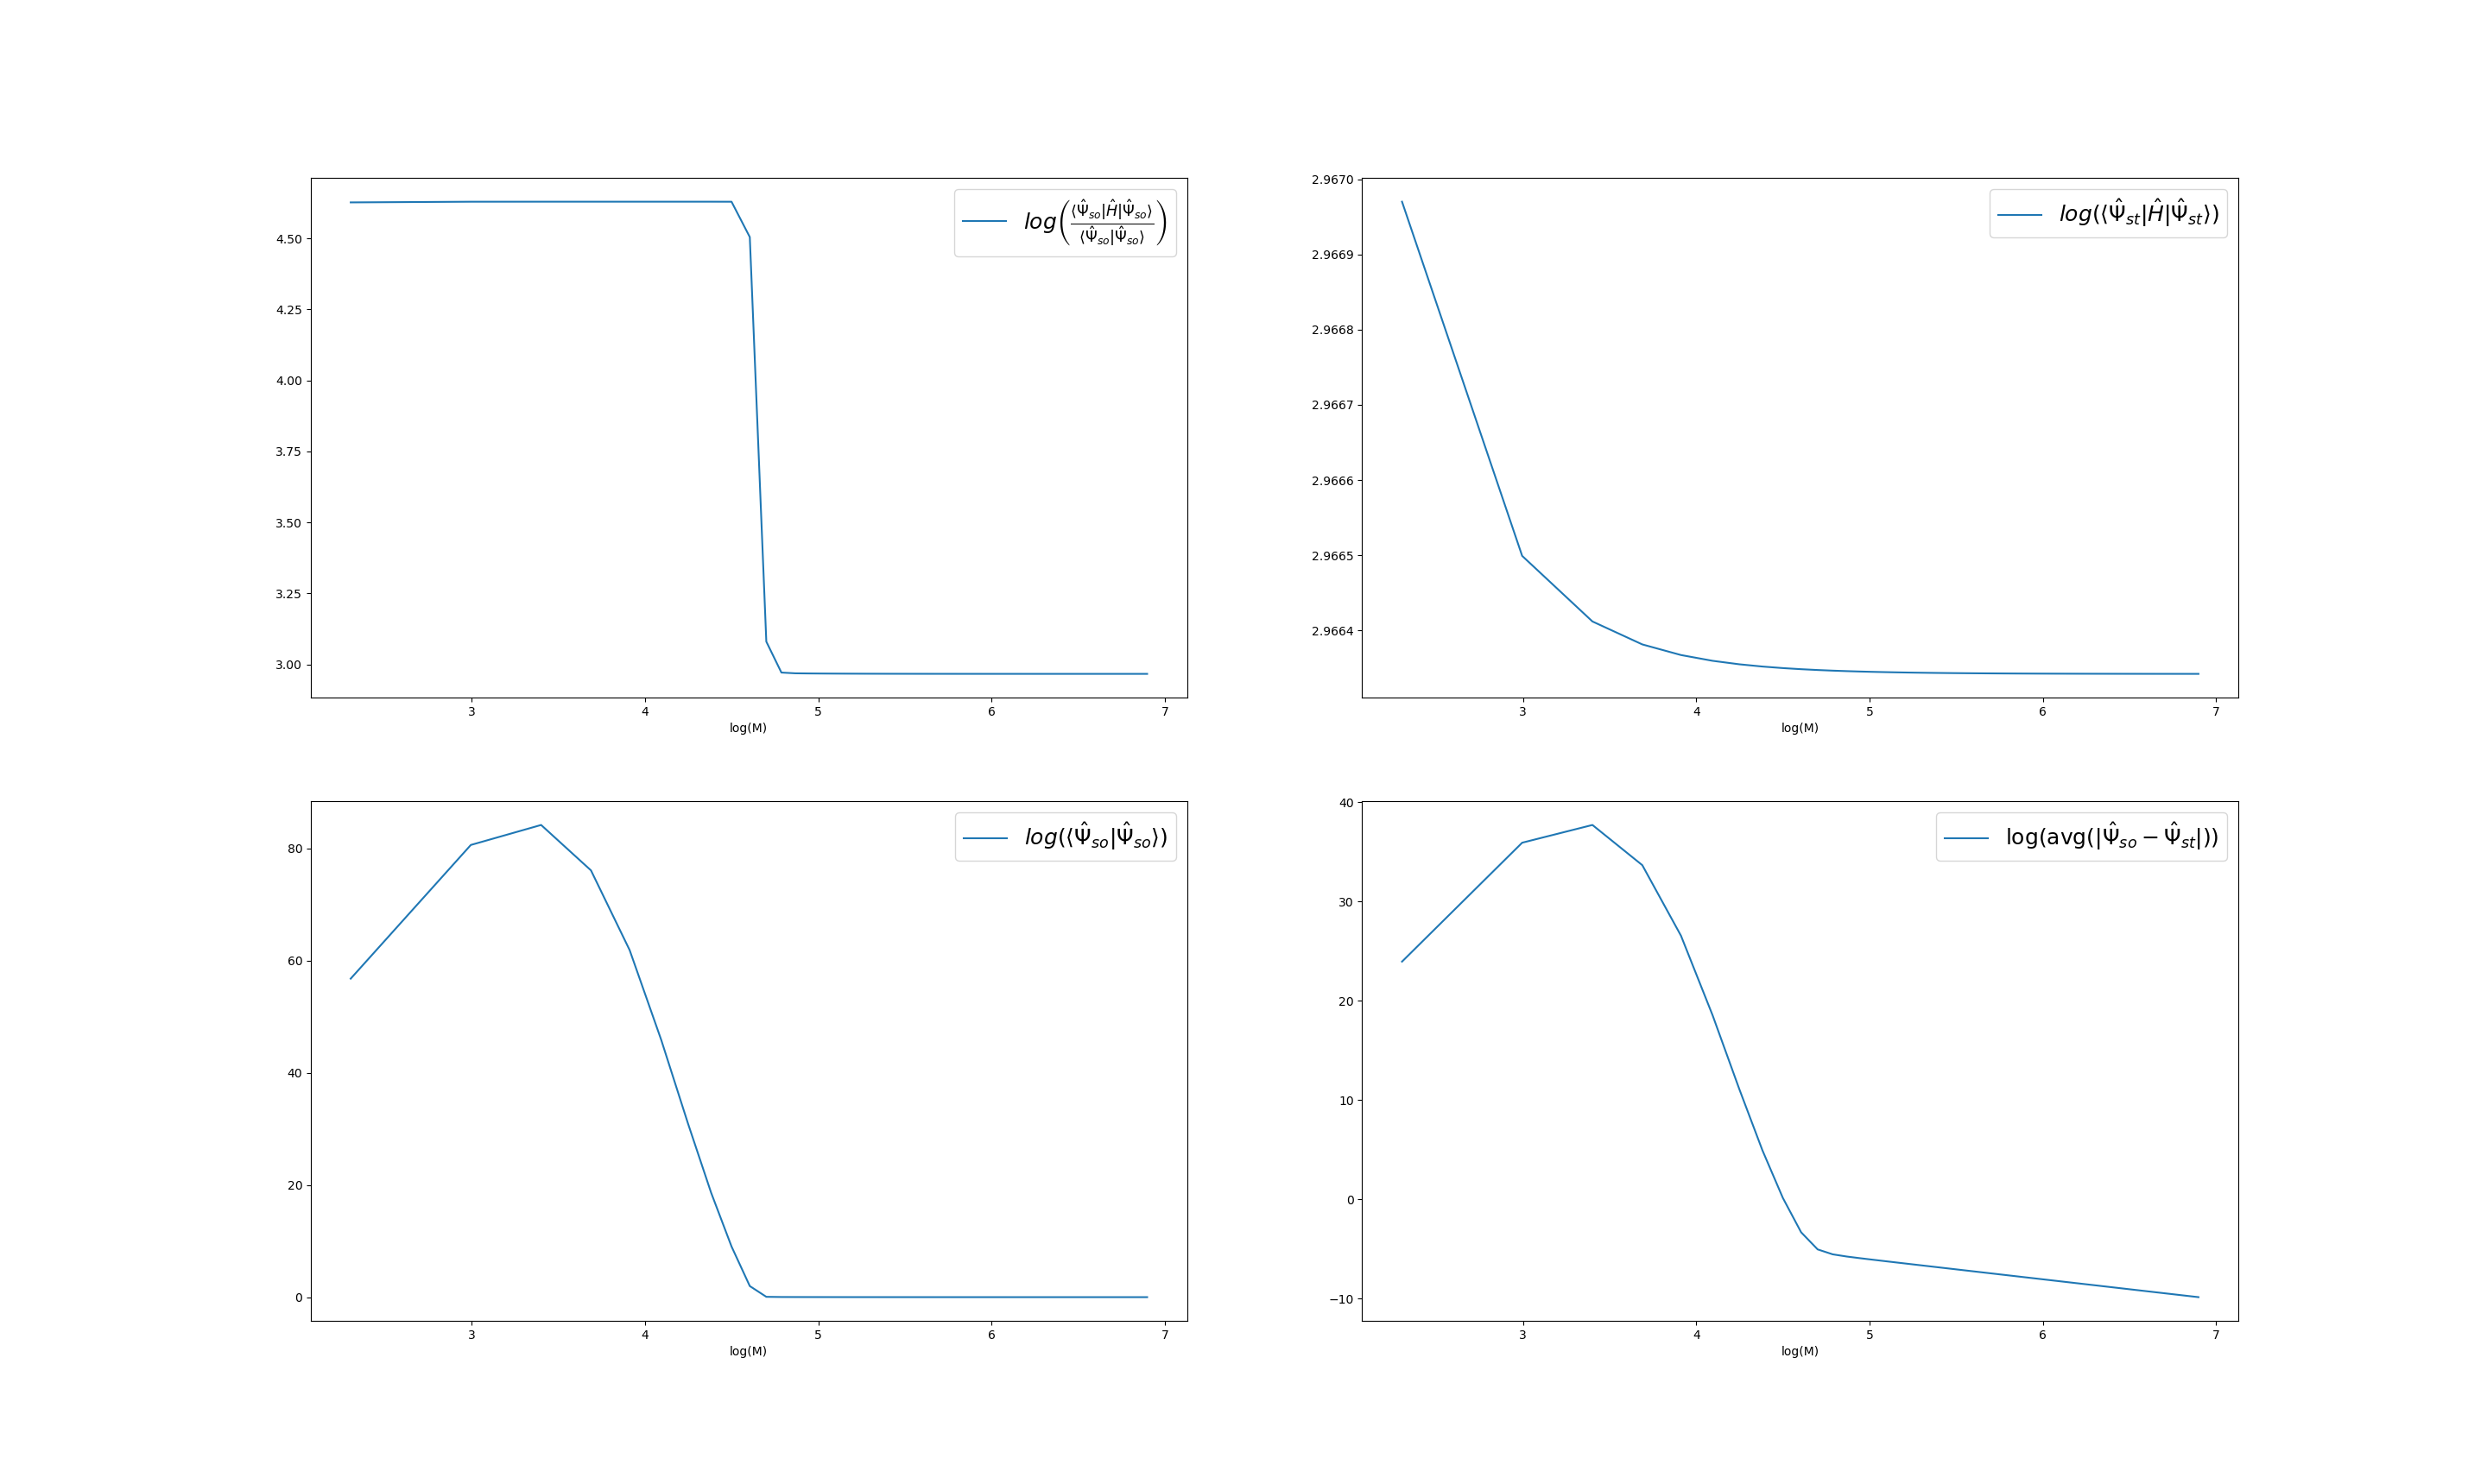
\includegraphics[width=.9\textwidth]{logvlog.png}
    \caption{log-log plot for $M\in[10, 990]$ }
\end{figure}\noindent\newline
When looking at higher values of M we can see the predicted linear plot for the difference between the two integrators implying the relationship $\ket{\Psi_{so}(t)}-\ket{\Psi_{st}(t)}\sim\tau^2$. For the other graphs we were not able to determine the relationship with tau, even for higher values of M.
\begin{figure}[!h]
    \centering
    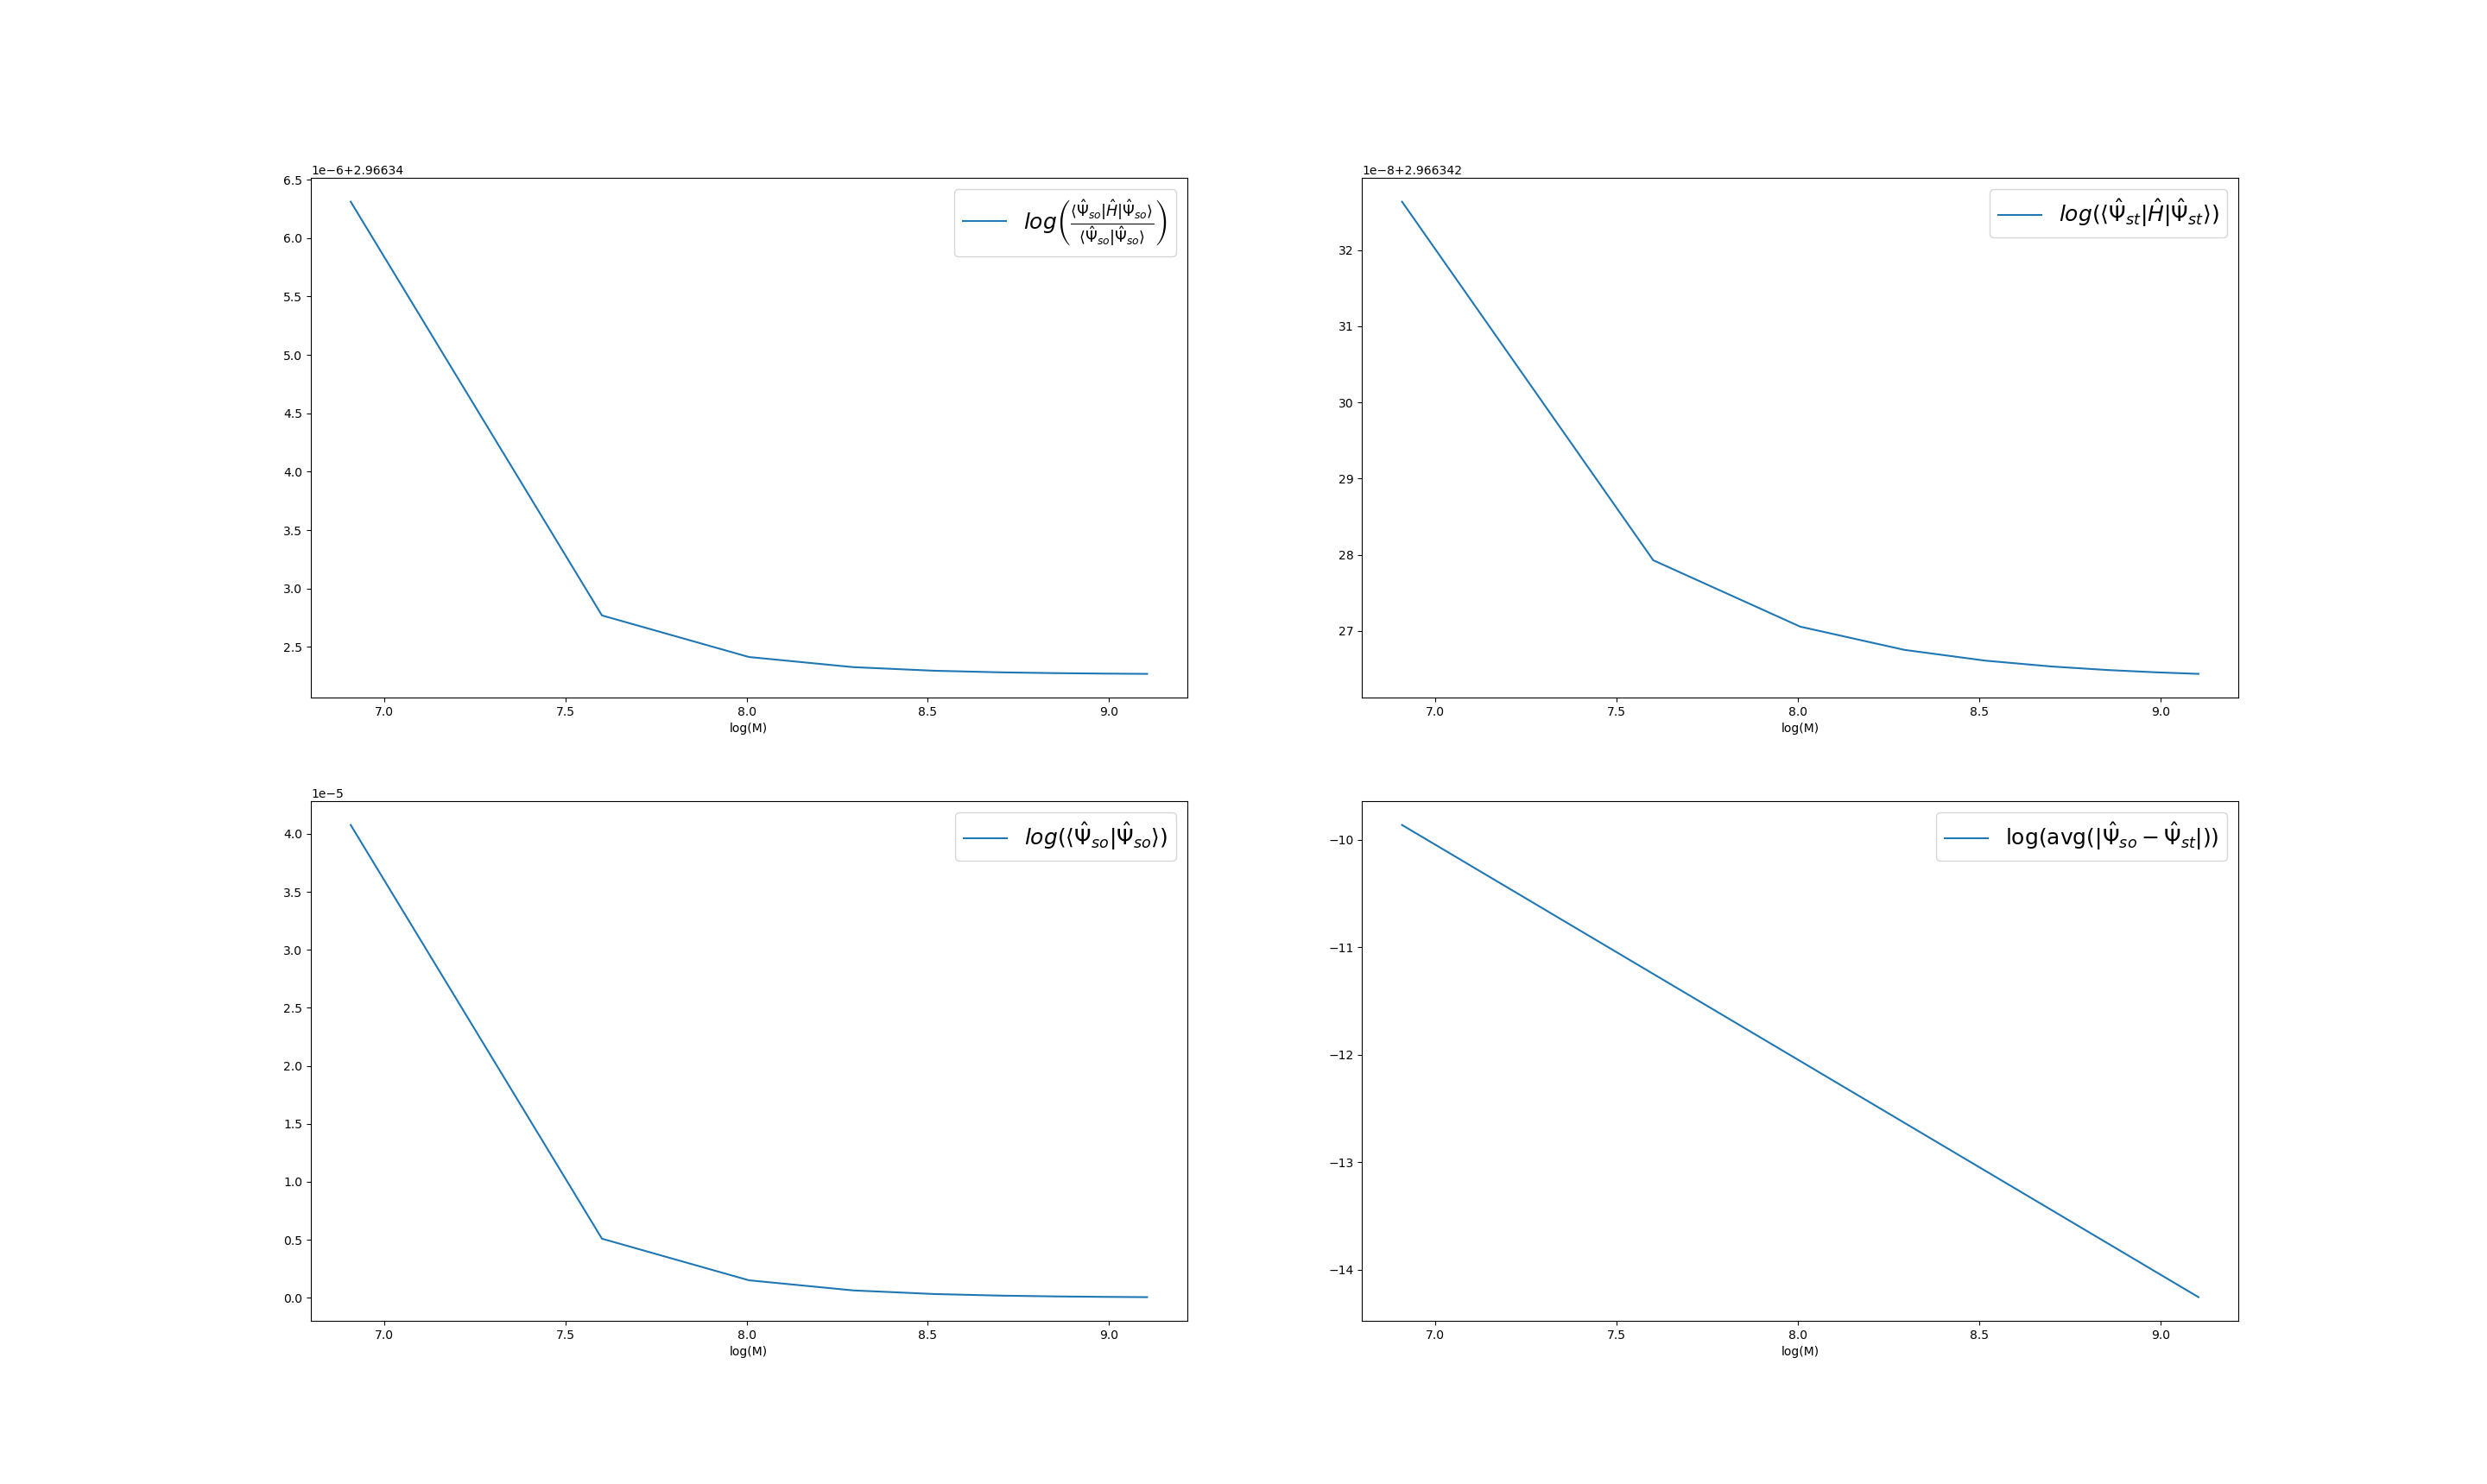
\includegraphics[width=.9\textwidth]{plots_for_1000M9000.png}
    \caption{log-log plot for $M\in[1000, 9000]$ }
\end{figure}\noindent\newline





\section{Appendix} \label{sec:appendix}

	\begin{figure}[h]	
	\begin{center}	
	\subfigure[Random input wavefunction]{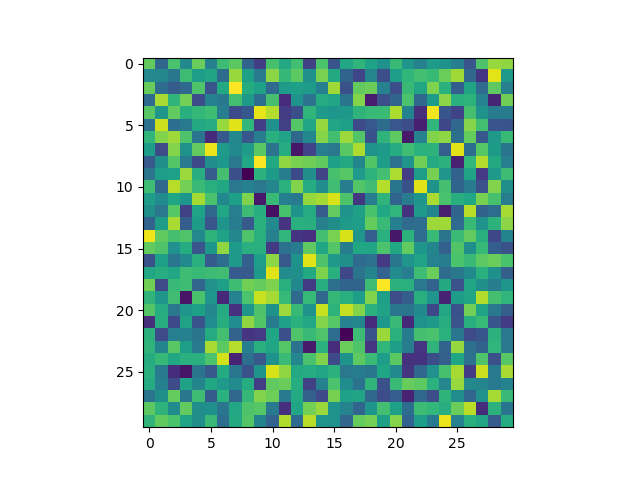
\includegraphics[width=0.35\textwidth]{function1_ABS.png}}
    \subfigure[Potential]
    {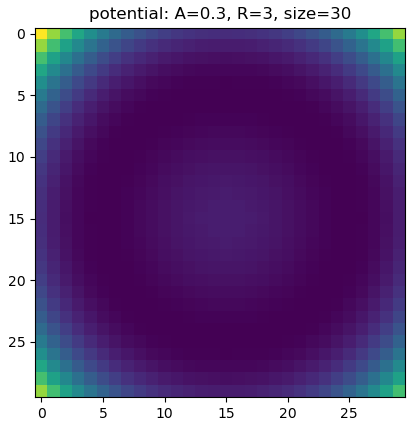
\includegraphics[width=0.35\textwidth]{potential2.png}}
    \subfigure[Second-order integration]
    {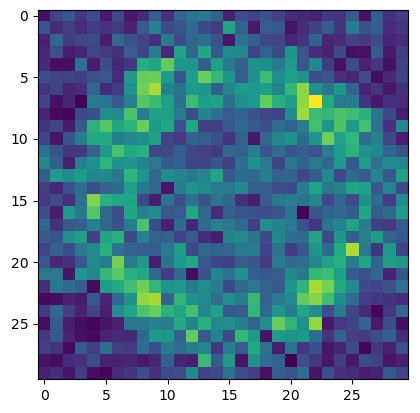
\includegraphics[width=0.35\textwidth]{so-integrator1_ABS.png}}
	\caption{Tests with (a) random 2D wavefunction, (b) resulting potential and (c) the following time evolution with the second-order integrator after a certain amount of time steps M (not known anymore, but around 2000 with T=2)}
	\label{fig:2D-so_integr}
	\end{center} 
	\end{figure}
	
	\begin{figure} [h] 
	\begin{center}
	\includegraphics[width=16cm]{"calc.jpeg"}
	\caption{Calculation of eigenvalues with pen and paper.}
		\label{fig:calc-eigenvalues}
	\end{center}
	\end{figure}
	
	
	\begin{figure} [h] 
	\begin{center}
	\includegraphics[width=16cm]{"animation-so-integratorEND.png
"}
	\caption{Test for a plot of the time evolution with the second-order integrator after a certain amount of time steps M for a 1D wavefunction which was set to be 1 at every lattice point, resulting in a symmetrical distribution.}
		\label{fig:1D-so_integr}
	\end{center}
	\end{figure}
    
	


	

	
	





	
\end{document}
